% Clean CV/Resume Template, by Bennet B <dev@bennet.cc>
% CC0, Public-Domain
% 
% Permission is hereby granted, free of charge, to any person obtaining a copy
% of this template and associated files (the "Template"), to deal
% in the Template without restriction, including without limitation the rights
% to use, copy, modify, merge, publish, distribute, sublicense, and/or sell
% copies of the Template, and to permit persons to whom the Template is
% furnished to do so, subject to the following conditions:
%
% The above copyright notice and this permission notice shall be included in all
% copies or substantial portions of the Template.
%
% THE TEMPLATE IS PROVIDED "AS IS", WITHOUT WARRANTY OF ANY KIND, EXPRESS OR
% IMPLIED, INCLUDING BUT NOT LIMITED TO THE WARRANTIES OF MERCHANTABILITY,
% FITNESS FOR A PARTICULAR PURPOSE AND NONINFRINGEMENT. IN NO EVENT SHALL THE
% AUTHORS OR COPYRIGHT HOLDERS BE LIABLE FOR ANY CLAIM, DAMAGES OR OTHER
% LIABILITY, WHETHER IN AN ACTION OF CONTRACT, TORT OR OTHERWISE, ARISING FROM,
% OUT OF OR IN CONNECTION WITH THE TEMPLATE OR THE USE OR OTHER DEALINGS IN THE
% TEMPLATE.
%
% based on Modern CV by Habib Semouma
% https://www.overleaf.com/latex/templates/modern-cv-slash-resume-template/vjrqdkpjckwj
%
%
% !TEX program = XeLaTeX
\documentclass[twoside]{article}

\usepackage{wallpaper}
\usepackage{geometry}
\usepackage[
    unicode=true,
    bookmarks=true,
    bookmarksnumbered=false,
    bookmarksopen=true,
    bookmarksopenlevel=1,
    breaklinks=false,
    pdfborder={0 0 0},
    backref=false,
    colorlinks=false
    ]{hyperref}
\usepackage{lastpage}
\usepackage{hyphenat}
\usepackage{hyphsubst}
\usepackage{tabularx}
\usepackage{moresize}
\usepackage[document]{ragged2e}
% \usepackage{parskip}

\usepackage[scaled]{helvet}
\usepackage{nopageno}
\usepackage{fontawesome5}
\usepackage{academicons}
\usepackage[defaultfam,tabular,oldstyle]{montserrat}
\usepackage[T1]{fontenc}
%\usepackage{afterpage}
\renewcommand*\oldstylenums[1]{{\fontfamily{Montserrat-TOsF}\selectfont #1}}
\usepackage{graphicx}
\usepackage{titlesec}
\usepackage{xcolor}
\usepackage{tikz}
\usepackage{color}

\setlength{\parindent}{0pt}
\titleformat{\section}{\normalfont}{}{0pt}{}

\renewcommand{\arraystretch}{1.4}

\setlength\fboxrule{0pt}
\setlength\fboxsep{12pt}
% \setlength{\parskip}{.5\baselineskip plus 2pt}
% \renewcommand{\baselinestretch}{1.1}
%\enlargethispage{-\baselineskip}
\titlespacing{\section}{0pt}{1.5ex plus .1ex minus .2ex}{1pc}

\newcolumntype{Y}{>{\RaggedRight\arraybackslash}X}

% Change PDF Meta Info here
\hypersetup{
    pdftitle={Morteza Montahaee - CV - English/German},
    pdfauthor={Morteza Montahaee},
    pdfsubject={CV},
    pdftitle={Mein CV erstellt mit LaTeX}
}

% Paper size
\geometry{
    a4paper,
    left=0pt,
    right=0pt,
    top=0pt,
    bottom=0pt,
    nohead,
    % includefoot,
    nomarginpar
}

% Background Color of the Sidebar Column
\definecolor{sidebg}{cmyk}{1, 0.02, 0, 0.56}
% Background Color of the Main Column
\definecolor{mainbg}{cmyk}{0, 0, 0.07, 0.04}

% Text Color of the Main Column
\definecolor{maintext}{cmyk}{1, 0.02, 0, 0.8}
% Text Color of the Sidebar Column
\definecolor{sidetext}{cmyk}{0, 0, 0.07, 0.04}

\pagecolor{mainbg}


\begin{document}
\setlength{\topskip}{0pt}\setlength{\footskip}{0pt}%
\fcolorbox{red}{sidebg}{%
    \begin{minipage}[t][\textheight-2\fboxsep-2\fboxrule][t]{\dimexpr0.40\textwidth-2\fboxrule-2\fboxsep\relax}
        \color{sidetext}
        %%%%%%%%%%%%%%%%%%%%%%%%%%%%%%%%%%%%%%%%%%%%%%%%%%%%
        % YOUR NAME, PRONOUNS, OCCUPATION(s), AND HEADSHOT
        {\bfseries\scshape\HUGE Morteza} \\
        {\bfseries\scshape\huge Monthaee} \qquad {\large\textbf{ Lebenslauf}}
        \vspace{.3cm} \\
        % Demo Subject, \\
        {\faStarOfLife{}  17/09/1984} 
        \\
        \begin{center}
            \begin{tikzpicture}
            \clip (0,0) circle (3cm) node[anchor=center] {\includegraphics[width=6cm]{portait_template.jpg}};
            \end{tikzpicture}
        \end{center}
        \vspace{.3cm}
        %%%%%%%%%%%%%%%%%%%%%%%%%%%%%%%%%%%%%%%%%%%%%%%%%%%%
        % YOUR PERSONAL INFROMATION
        \phantomsection{}
        \addcontentsline{toc}{section}{Personal info}
        \section*{\Large Kontakte}
        \begin{tabularx}{\textwidth}{cY}
            \faPhone{}      & \href{tel:+49 176 703 552 53}{+49 176 703 552 53} \\
            \faSkype{}      & \href{skype:Morteza Montahaee?chat}{Morteza Montahaee} \\
            \faEnvelope{}   & \href{mailto:morteza.montahaee@rwth-aachen.de}{morteza.montahaee@outlook.com} \\
            \faMapMarker{}  & \href{https://www.bing.com/maps?q=Otto+str+19+aachen\&FORM=AWRE}{Ottostr. 19, 52070 Aachen} \\
        \end{tabularx}
        \vspace{.3cm} \\
        \rule{\linewidth}{0.4pt} \\
        %%%%%%%%%%%%%%%%%%%%%%%%%%%%%%%%%%%%%%%%%%%%%%%%%%%%%%%%%
        % YOUR LINKS, YOU MAY ALSO ADD A PERSONAL WEBSITE OR PORTFOLIO
        \phantomsection{}
        \addcontentsline{toc}{section}{Links}
        \section*{\large Links}
        \begin{tabular}{cl}
        %    \faCode{}     & \href{https://example.com}{example.com}
            \faGithub{}   & \href{https://github.com/montahaee}{montahaee} \\
            \faGlobe{} & \href{https://montahaee.github.io/}{montahaee.github.io} \\
            % \faXing{}     & \href{https://www.xing.com/profile/Mor_Mon7373990/cv}{/Mor\_Mon7373990} \\
            
\includegraphics[width=1.25em]{icon-twitterx-500.png} &  \href{https://x.com/Mor_Montahaee}{Mor\_Montahaee} \\
        \end{tabular}
        \vspace{10pt} \\
        \rule{\linewidth}{0.4pt} \\
        %%%%%%%%%%%%%%%%%%%%%%%%%%%%%%%%%%%%%%%%%%%%%%%%%%%%%%%%%%%%
        % YOUR SKILLS
        % Add/Remove as seen fit, Icons: https://packages.oth-regensburg.de/ctan/fonts/fontawesome5/doc/fontawesome5.pdf
        \phantomsection{}
        \addcontentsline{toc}{section}{Skills}
        \section*{\large Skills}

        \begin{tabularx}{\textwidth}{cY}
            \faCode{}        & C++, C, Python, Bash, PHP, Javascript, C\#, Java, MariaDB, MySQL, Visual Basic \\
            \faPen*{}        & \LaTeX, Liquid, HTML, CSS, SHACL \\
            \faFont{}        & \{MS, Libre\} Office, Vim, PDF-XChange,  Adobe Acrobat \\
            \faCogs{}        & Dual (Windows, Linux) \\
            \faLaptopCode{}  & IntelliJ, Rider, Visual Studio/Code, PyCharm,  CLion, DataGrip, MATLAB\\
            \faToolbox{}     & Docker, Enterprise Architect, Git
        \end{tabularx}
        \vspace{1pt} \\
        \rule{\linewidth}{0.4pt}
        %%%%%%%%%%%%%%%%%%%%%%%%%%%%%%%%%%%%%%%%%%%%%%%%%%%%%%%%%%%%%%%%
        % GRADESCALE (if nesseary, e.g. if you apply abroad, where scales 
        % are different. You should at least provide, what the best possible
        % grade and what the worst possible grade is)
        \vfill
        \begin{center}
            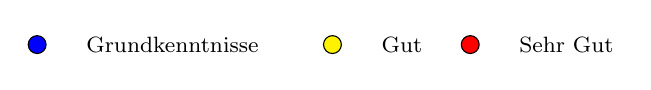
\begin{tikzpicture}
                % Low-level
                \draw[fill=blue] (0,0) circle (0.75ex);
                \node[right] at (0.5,0) {\footnotesize Grundkenntnisse};

                % Mid-level
                \draw[fill=yellow] (3.75,0) circle (0.75ex);
                \node[right] at (4.25,0) {\footnotesize Gut};

                % High-level
                \draw[fill=red] (5.5,0) circle (0.75ex);
                \node[right] at (6.00,0) {\footnotesize Sehr Gut};
            \end{tikzpicture}
        \end{center}
        {\tiny Grade scale: (1) very good $\approx$91\%-100\%, (2) good $\approx$81\%-90\%, (3) satisfactory $\approx$66\%-80\%, (4) sufficient $\approx$50\%-65\%, (5) failed $\approx$0\%-49\%}
    \end{minipage}
}
\hfill
\fcolorbox{red}{mainbg}{%
    \begin{minipage}[t][\dimexpr\textheight-2\fboxrule-2\fboxsep\relax][t]{\dimexpr0.6\textwidth-2\fboxrule-2\fboxsep\relax}
        \color{maintext}
        %%%%%%%%%%%%%%%%%%%%%%%%%%%%%%%%%%%%%%%%%%%%%%%%%%%%%%%%%%%
        % EDUCATION
        \phantomsection{}
        \addcontentsline{toc}{section}{Education}
        \section*{\scshape\Large Education \rule{\linewidth}{0.4pt}}
%
        {\large \textbf{Management \& Business Administration, Sample University\\ (Graduate Degree)}} \\
        {\scshape\fontseries{light}\selectfont\footnotesize Springfield \qquad Oct 2013 \textendash{} Nov 2016} \\
        {Degree: Diploma of Business} \\[1ex]
        {Grade: 2.6} \\[1ex]
        {\footnotesize Subsidiary subject: Psychology} \\
        {\footnotesize In-depth study: Thievery} \\
        {\footnotesize Thesis subject: ultrices gravida dictum fusce} \\[2ex]

        {\large \textbf{Potenti nullam \textendash{} sodales ut, Some School\\ (Professional Training with A-Levels)}} \\
        {\scshape\fontseries{light}\selectfont\footnotesize Miami \qquad Sep 2010 \textendash{} Sep 2013} \\
        {Degrees: Potenti nullam \& A-Levels\\ (General higher education entrance qualification)} \\[1ex]
        {Vocational Grades: interdisciplinary 1.7, subject-specific 1.1} \\
        {Grammar School Grade: 3.4} \\[1ex]
        {\footnotesize Project subject: sit amet nulla facilisi} \\[2ex]

        {\large \textbf{School Education, Middle school}} \\
        {\scshape\fontseries{light}\selectfont\footnotesize New York \qquad Sep 2005 \textendash{} Jun 2010} \\
        {Degree: Secondary school leaving certificate} \\[1ex]
        {Grade: 2.5} \\[1ex]
        {\footnotesize Elective Courses: Chemistry, Engineering, Art} \\
         \vspace{+7pt}
        %%%%%%%%%%%%%%%%%%%%%%%%%%%%%%%%%%%%%%%%%%%%%%%%%%%%%%%%%%
        % WORK EXPERIENCE
        \phantomsection{}
        \addcontentsline{toc}{section}{Work Experience}
        \section*{\scshape\Large Work Experience \rule{\linewidth}{0.4pt}}
%
        {\large \textbf{United Staats Government}} \\
        {{\fontseries{medium}\selectfont Full-time, President}} \\
        \faCalendar {} {\scshape\fontseries{light}\selectfont\footnotesize Jan 2016 \textendash{} Nov 2020}
        \begin{itemize}
            \setlength{\itemsep}{-3pt}
            \item Do stuff
            \begin{itemize}
                \item That included Stuff
                \item and more Stuff
            \end{itemize}
            \item Other Task
        \end{itemize}
%
        {\large \textbf{McKienze Ltd}} \\
        {{\fontseries{medium}\selectfont Part-time, Thieve}} \\
        {\scshape\fontseries{light}\selectfont\footnotesize Oct 2013 \textendash{} Nov 2016}
        \begin{itemize}
            \setlength{\itemsep}{-3pt}
            \item Do stuff
            \begin{itemize}
                \item That included Stuff
                \item and more Stuff
            \end{itemize}
            \item Other Task
            \begin{itemize}
                \item That included more Stuff
                \item and other more different Stuff
            \end{itemize}
            \item tellus elementum sagittis vitae et
            \item aliquam sem et tortor consequat
            \item ullamcorper velit sed ullamcorper morbi tincidunt
            \item rhoncus est pellentesque elit ullamcorper dignissim
        \end{itemize}
%
        {\large \textbf{ACME Corp}}\\
        {{\fontseries{medium}\selectfont Traineeship, Occupation}}\\
        {\scshape\fontseries{light}\selectfont\footnotesize Aug 2010 \textendash{} Oct 2013}
        \begin{itemize}
            \setlength{\itemsep}{-4pt}
            \item massa tempor nec feugiat nisl pretium fusce id
        \end{itemize}
        \vfill%
        {\hfill\small\fontseries{extralight}\selectfont Page \thepage of \pageref{LastPage}\hfill}
    \end{minipage}
}%

\newpage
%%%%%%%%%%%%%%%%%%%%%%%%%%%%%%%%%
% PAGE 2
%%%%%%%%%%%%%%%%%%%%%%%%%%%%%%%%%
\fcolorbox{red}{mainbg}{%
    \begin{minipage}[t][\dimexpr\textheight-2\fboxrule-2\fboxsep\relax][t]{\dimexpr0.6\textwidth-2\fboxrule-2\fboxsep\relax}
        \color{maintext}
        % \vspace{.6cm}
        %%%%%%%%%%%%%%%%%%%%%%%%%%%%%%%%%%%%%%%%%%%%%%%%
        % PROJECTS
        \phantomsection
        \addcontentsline{toc}{section}{Projects}
        \section*{\scshape\Large Projects \rule{\linewidth}{0.4pt}}
        \begin{justify}
        \setlength{\parindent}{0pt}
        {\large \textbf{Quis blandit turpis}} \\
        {\scshape\fontseries{light}\selectfont\footnotesize Acme Corp \qquad 2017} \\
        Lorem ipsum dolor sit amet, consectetur adipiscing elit, sed do eiusmod tempor incididunt ut labore et dolore magna aliqua. Tincidunt praesent semper feugiat nibh sed pulvinar. Tristique nulla aliquet enim tortor at auctor. \\[1ex]
        Skill 1, Skill 2, Skill 3 \\

        {\large \textbf{Lacus laoreet non}} \\
        {\scshape\fontseries{light}\selectfont\footnotesize Acme Corp \qquad 2018} \\
        Pellentesque elit ullamcorper dignissim cras tincidunt. Sit amet commodo nulla facilisi nullam vehicula ipsum. Blandit cursus risus at ultrices mi tempus imperdiet. Lectus sit amet est placerat in egestas erat.\\[1ex]
        Skill 1, Skill 2, Skill 3, \LaTeX \\

        {\large \textbf{Viverra maecenas accumsan lacus}} \\
        {\scshape\fontseries{light}\selectfont\footnotesize Private \qquad 2022 and ongoing} \\
        Quisque non tellus orci ac auctor augue mauris augue neque. Sit amet luctus venenatis lectus magna fringilla urna porttitor rhoncus. Proin nibh nisl condimentum id venenatis a condimentum vitae sapien. \\[1ex]
        Skill 1, Skill 2, Skill 3 \\
        
        {\large \textbf{Ut faucibus pulvinar elementum}} \\
        {\scshape\fontseries{light}\selectfont\footnotesize TU Dresden \qquad 2022} \\
        Proin nibh nisl condimentum id venenatis a condimentum vitae sapien. Amet aliquam id diam maecenas ultricies mi eget. Viverra maecenas accumsan lacus vel facilisis volutpat. \\[1ex]
        Skill 1, Skill 2, Skill 3 \\

        {\large \textbf{Quisque non tellus orci}} \\
        {\scshape\fontseries{light}\selectfont\footnotesize ACME Corp. \qquad 2023} \\
        Viverra maecenas accumsan lacus vel facilisis volutpat. Tortor condimentum lacinia quis vel eros donec ac odio tempor. Ultricies lacus sed turpis tincidunt id aliquet risus. \\[1ex]
        Skill 1, Skill 2, Skill 3 \\
        
        {\large \textbf{Amet consectetur adipiscing elit}} \\
        {\scshape\fontseries{light}\selectfont\footnotesize ACME Corp \qquad 2023} \\
        Eget lorem dolor sed viverra. Eleifend donec pretium vulputate sapien. Pellentesque pulvinar pellentesque habitant morbi tristique senectus et netus et. Augue neque gravida in fermentum et. Ullamcorper velit sed ullamcorper morbi tincidunt ornare massa eget egestas. \\[1ex]
        Skill 1, Skill 2, Skill 3 \\
        
        {\large \textbf{Augue neque gravida in fermentum}} \\
        {\scshape\fontseries{light}\selectfont\footnotesize Sample Uni \qquad 2023} \\
        met aliquam id diam maecenas ultricies mi eget. Viverra maecenas accumsan lacus vel facilisis volutpat. Tortor condimentum lacinia quis vel eros donec ac odio tempor. Ultricies lacus sed turpis tincidunt id aliquet risus. \\[1ex]
        Skill 1, Skill 2, Skill 3, \LaTeX 
        \end{justify}
        \vfill%
        {\hfill\small\fontseries{extralight}\selectfont Page \thepage of \pageref{LastPage}\hfill}
    \end{minipage}
}
\hfill%
\fcolorbox{red}{sidebg}{%
    \begin{minipage}[t][\dimexpr\textheight-2\fboxrule-2\fboxsep\relax][t]{\dimexpr0.4\textwidth-2\fboxrule-2\fboxsep\relax}
        \color{sidetext}
        % \vspace{.5cm}
        %%%%%%%%%%%%%%%%%%%%%%%%%%%%%%%%%%%%%%%%%%%%%%%%%%%%%%%%
        % YOUR NAME AND PREFERED PRONOUS AGAIN AS HEADER
        {\bfseries\scshape\HUGE Morteza} \\
        {\bfseries\scshape\Huge Montahaee} \qquad {they/them}
        \vspace{.3cm} \\
        %%%%%%%%%%%%%%%%%%%%%%%%%%%%%%%%%%%%%%%%%%%%%%%%%%%%%%%%%%
        % LANGUAGES
        \phantomsection
        \addcontentsline{toc}{section}{Languages}
        \section*{\large Languages}
        \begin{tabular}{cl}
            \faLanguage{} & Lorem ipsum (Mothertounge) \\
            \faLanguage{} & English (Fluent)
        \end{tabular}
        \vspace{.3cm}
        \\
        \rule{\linewidth}{0.4pt}
        \\
        %%%%%%%%%%%%%%%%%%%%%%%%%%%%%%%%%%%%%%%%%%%%%%%%%%%%%%%%%%%%
        % CERTIFICATES AND AWARDS RECEIVED
        \phantomsection
        \addcontentsline{toc}{section}{Certificates and Prizes}
        \section*{\large Certificates and Prizes}
        \begin{tabularx}{\textwidth}{cY}
            2010 & Etiam tempor orci eu \\
            2010 & Quam nulla porttitor massa \textemdash{} 3\textsuperscript{rd} place \\
            2011 & Quis imperdiet massa tincidunt \textemdash{} 3\textsuperscript{rd} place \\
            2016 & Vestibulum sed arcu non odio euismod \\
            2016 & Non enim praesent elementum facilisis \\
            2016 & Blandit libero volutpat sed cras \\
            2016 & Eget dolor morbi non arcu \\
        \end{tabularx}
        \vspace{.3cm}
        \\
        \rule{\linewidth}{0.4pt}
        \\
        %%%%%%%%%%%%%%%%%%%%%%%%%%%%%%%%%%%%%%%%%%%%
        % HOBBIES
        % Change Icons here https://packages.oth-regensburg.de/ctan/fonts/fontawesome5/doc/fontawesome5.pdf
        \phantomsection
        \addcontentsline{toc}{section}{Hobbies}
        \section*{\large Hobbies}
        \begin{tabularx}{\textwidth}{cY}
            \faCamera{} & Fringilla \\
            \faCogs{} & Id eu nisl nunc mi ipsum \\
        \end{tabularx}
        \vspace{.3cm}
        \\
        \rule{\linewidth}{0.4pt}
    \end{minipage}%
}%
%    \cleardoubleemptypage
% \afterpage{\null\newpage}
\end{document}